\documentclass[11pt,a4paper]{article}

% -------------------------------------------------
% Packages
% -------------------------------------------------
\usepackage[T1]{fontenc}
\usepackage[utf8]{inputenc}
\usepackage{amsmath}
% TikZ diagrams
\usepackage{tikz}
\usetikzlibrary{arrows.meta, positioning, shapes.geometric}
\usepackage{pgfplots}
\pgfplotsset{compat=1.18}
\usepackage{float}
\usepackage[margin=1in]{geometry}
\usepackage{microtype}
\usepackage{graphicx}
\usepackage{booktabs}
\usepackage{array}
\usepackage{tabularx}
\usepackage{url}
\usepackage{hyperref}
\usepackage{xspace}
\newcommand{\vcache}{value cache\xspace}

% Long monospaced identifiers cannot be hyphenated. Allow some extra
% inter-word stretch before a line is allowed to overflow the margin.
\setlength{\emergencystretch}{2em}


\hypersetup{
    colorlinks=true,
    linkcolor=blue,
    citecolor=blue,
    urlcolor=blue
}

% -------------------------------------------------
% Title
% -------------------------------------------------
\title{
    \textbf{Design and Evaluation of Value Prediction
    Mechanisms in gem5 MinorCPU}
}

\author{
    \textbf{Ayush Gangal}\\
    \textbf{Department of Computer Science and Engineering}\\
    \textbf{Indian Institute of Technology Madras}\\
    \textbf{Advisor: Prof. Gopalakrishnan Srinivasan}
}

\date{}

% -------------------------------------------------
% Document
% -------------------------------------------------
\begin{document}

\maketitle

\begin{abstract}
In an in-order processor, a load that is waiting for memory can hold up the instructions after it. Value prediction tries to fix this by guessing a result early, so that dependent instructions can start sooner. In this project, value prediction is added to gem5's MinorCPU, following a 2025 HPCA paper on value prediction for in-order cores.

Last Value Prediction (LVP), an address predictor called ASTRA, and a small value cache are explored. V-ASTRA takes ASTRA's guess for a load's base address, adds the offset from the instruction, and reads the value from the value cache, so the load can skip the normal memory access. This work checks for two ways of letting dependent instructions start earlier, and built a version of the paper's META predictor, which picks at most one of LVP or V-ASTRA for each load that depends on an earlier load. An extra experimental mode lets loads predicted by LVP help train ASTRA and become V-ASTRA candidates.

The mechanisms are validated with directed RISC-V tests and measured performance on small deterministic microbenchmarks. The benefit depends a lot on the workload. META matches V-ASTRA on several workloads, but on the random-base workload it reduces cycles by 30.27\%, while V-ASTRA alone reduces them by 48.75\%. The experimental candidate mode brings this up to 50.80\%.
\end{abstract}

{\raggedright\noindent\textbf{Source code:} \url{https://github.com/ayushgangal/gem5-minorcpu-value-prediction}
(branch \texttt{astra-vastra-dev})\par}

\newpage

\tableofcontents
\newpage

\section{Introduction}

Modern processors often stall because of dependencies between
instructions. Value prediction tries to reduce
this delay by guessing an instruction's result before it is
available, so that dependent operations can start earlier. A wrong
guess must be detected and handled without breaking correctness.

This project builds on
``Architecting Value Prediction around In-Order Execution''
\cite{ravenel2025architecting}. The paper studies value prediction in
in-order processors using Last Value Prediction (LVP), ASTRA-based
load-base prediction, and V-ASTRA. V-ASTRA combines a predicted load
base with a dedicated value cache, so load values are available
earlier. The paper also introduces META, which coordinates LVP and
V-ASTRA. It further describes address compression, store tracking,
scoreboard replay, and a speculative L0 minicache.

My objective was to implement and evaluate similar mechanisms in
gem5 using MinorCPU. MinorCPU differs from the processor in the
original study, so I had to change how it handles loads, their
dependent instructions, and recovery from wrong predictions.

I implemented an LVP predictor and an ASTRA-based predictor for load
base addresses. V-ASTRA adds the instruction's offset to the predicted
base and reads the load value from a small value cache. When a set of
safety checks passes, the load can skip its normal memory request.

On top of these, I tried two ways of letting dependent instructions start
earlier. Design~A only releases the scoreboard dependency, while
Design~B also forwards the validated value. I also adapted META to
choose at most one of LVP or V-ASTRA for each dependent load. Finally,
an experimental option lets loads served by LVP feed their base
addresses to ASTRA, both for training and for V-ASTRA candidacy.

I evaluated the implementation using directed RISC-V regression
tests and deterministic microbenchmarks. The tests check that predictions,
bypasses, and recovery behave correctly. The performance experiments
compare no prediction (NP), LVP, V-ASTRA, and META on workloads with
different address, value, and dependency patterns, including the
experimental provisional-base modes.

\newpage
\section{Background}

\subsection{Last Value Prediction}

The simplest guess for an instruction's result is the value it
produced the last time it ran. Last Value Prediction (LVP) uses
exactly this guess. It is a computational
predictor that applies the identity function to the last observed
value~\cite{ravenel2025architecting}. Predictions are usually
associated with static instructions using their PCs, so observations
from earlier executions can be reused.

Instruction values may change across executions, so LVP uses a
confidence counter to decide when a prediction is admitted. The design
in \cite{ravenel2025architecting} uses a two-bit saturating counter,
incremented on correct predictions and decremented on incorrect
ones. A prediction is admitted only when the counter is saturated.
In this implementation, the admission threshold is configurable.
The counter is updated for every eligible load that completes,
whether or not a prediction was made or used. This means entries
below the threshold can keep gaining confidence.

Accuracy alone is not enough, and neither is coverage. A predictor with high accuracy but few
predictions may give little benefit. A predictor with high coverage
may not help if the predicted instructions are not on critical
dependency chains.

LVP is especially relevant to in-order processors, where a
long-latency load can delay younger dependent instructions. A
predicted value lets eligible consumers, including dependent memory
operations, proceed before the producer completes. Memory operations
that would otherwise wait for one another can then overlap.

The producer still runs, and its real value is checked against the
prediction when it completes. If an
incorrect value was used, the processor must recover the affected
younger instructions to keep the architectural state correct.

\subsection{ASTRA Address Prediction}

Besides values, the paper also predicts load addresses, using a
predictor called ASTRA (Address Stride Alias)~\cite{ravenel2025architecting}. It uses an order-1 differential
finite-context method (D-FCM), with two modifications: it uses the
last observed stride directly as history, and its tables are untagged.

ASTRA is indexed by load PC. Its Last Address Table (LAT) stores
the last committed virtual address and signed stride for each
entry. The stride indexes a second table, Stride$\rightarrow$Stride
(SS), which gives the stride that is added to the LAT address to
form the predicted address. When a load retires, ASTRA computes the
new stride, updates the corresponding SS entry, and records the
committed address and stride in the LAT.

Because the SS table is untagged, loads that see the same stride
share entries. The paper uses this aliasing on purpose. When one
load updates an entry, other loads can use it to predict a new
access pattern. As a result, ASTRA favors prediction
coverage over accuracy, and it depends on address validation before
a prediction is used (Section~\ref{sec:bg-vastra}).

The original ASTRA predicts the complete load address. V-ASTRA
instead predicts the load's base-register value and adds the
instruction displacement. This project implements the base-address
form, so its LAT stores the base-register value rather than the
complete effective address (Section~\ref{sec:impl-astra}). ASTRA
predicts an address, not the loaded data. Getting the load value
requires V-ASTRA's separate value cache.

\subsection{V-ASTRA and the Value Cache}
\label{sec:bg-vastra}

To supply the data itself, V-ASTRA (Value-Address Stride Alias)
uses ASTRA's predicted address to read a dedicated value cache, which
stores previously observed load values. In the paper, the value cache holds 4\,KiB of data
in 16-byte entries. Loads allocate entries at commit, while stores
update matching entries without allocating new ones.

V-ASTRA predicts a load's base address and adds the displacement
from the decoded instruction to get its effective address.
The paper checks the predicted base at issue by comparing it
with the actual base-register value. A wrong prediction is
therefore rejected before it is used, so V-ASTRA needs neither a
confidence counter nor recovery from value mispredictions.

For a bypass to be safe, the value cache must also contain the
requested bytes, and no older in-flight store may modify them. The
paper uses a counting Bloom filter to detect stores that might
conflict, and an invalidation FIFO to handle older stores that
issue after a prediction. When all checks succeed, the load skips
the L1D access and its dependents can issue in the same cycle~\cite{ravenel2025architecting}.

The implementation splits the check into two stages and replaces the Bloom
filter and FIFO with an exact scan of older stores
(Section~\ref{sec:impl-vcache}).

\subsection{Dependency Handling}

When an instruction needs a value from an earlier instruction, it
has to wait for that producer. In an in-order processor,
a consumer waiting for a long-latency load can also delay younger
independent instructions, because issue follows program order. Under
stall-on-use, a dependent instruction cannot issue until the
producer's value becomes available.

Two mechanisms can reduce this delay. Dependency release
makes the consumer eligible to issue earlier but does not provide
the required value. Value forwarding supplies the producer's
value directly, so an eligible consumer can proceed before the
producer completes. In the paper, issue-time V-ASTRA validation
lets dependents issue in the same cycle as the load. MinorCPU
handles operands differently. Ordinary non-memory instructions read
their operands at commit, while memory operations can issue to
the LSQ earlier (Section~\ref{sec:bg-minor}). For this reason, the
forwarding mechanism in this implementation is restricted to eligible
dependent loads.

\subsection{META Selection}

Some loads have predictable addresses, while others have predictable
values. ASTRA/V-ASTRA targets the first kind and LVP the second, so
META combines them to improve
prediction coverage \cite{ravenel2025architecting}.

In the original design, both predictors operate in parallel, and
META selects a prediction at issue time. A validated V-ASTRA value
is preferred when the predicted base is correct and the requested
data is available in the value cache. Otherwise, META uses an
LVP prediction if its confidence counter is saturated. If neither
is available, the load is not predicted. Both predictors are updated
when the load retires~\cite{ravenel2025architecting}.

V-ASTRA
validates its address before use, whereas LVP remains speculative
until the actual value is available. So an incorrect LVP prediction
needs recovery only if it was used. The paper replays younger
instructions through the scoreboard, while the implementation squashes and
refetches them (Section~\ref{sec:impl-meta}).

\subsection{gem5 MinorCPU}
\label{sec:bg-minor}

All of this work is done in MinorCPU, gem5's in-order processor
model~\cite{gem5}. Its four pipeline stages are Fetch1 (instruction fetch),
Fetch2 (instruction separation and branch prediction), Decode, and
Execute. Execute contains the functional-unit pipelines, in-flight
instruction queue, commit logic, and load-store queue (LSQ).

Instructions issue to functional units in program order when their
source registers are ready according to the scoreboard. The
scoreboard tracks expected result availability and the latest
in-flight writer of each register, but does not hold register values.
Results are written to architectural registers at commit, also in
program order.

Memory instructions can compute their addresses and enter the LSQ
before they reach the head of the in-flight queue. However, they
issue one at a time, and ordinarily only after the instructions that
produce their sources have committed. Loads write their destination
registers at commit. Branches are resolved in Execute, and a
misprediction causes younger wrong-path instructions to be discarded.

The memory functional unit uses \texttt{extraAssumedLat} to estimate
when dependents may issue. With the default setting, dependents may
issue after an assumed load latency, but they still wait for the
producer to commit before executing. Setting this latency to zero
enables the stall-on-use configuration, in which dependents wait for
commit before issuing.

\newpage
\section{Implementation}

\subsection{Implementation Environment}
\label{sec:impl-env}

The implementation is based on gem5 version 23.0.0.1, and was developed on a separate branch. The simulator is built for the RISC-V ISA. All experiments use
syscall-emulation mode with a single \texttt{RiscvMinorCPU} that has
one hardware thread. The workloads are statically linked
RISC-V programs built for the \texttt{rv64g} ISA.

The baseline configuration models a 1\,GHz \texttt{RiscvMinorCPU}
with timing memory accesses and 64-byte cache lines. The L1
instruction cache is 32\,KiB and 4-way. The L1 data cache is 64\,KiB
and 4-way, with 16 MSHRs and a stride prefetcher. The L2 cache is
256\,KiB and 8-way, with 20 MSHRs and an AMPM prefetcher, and main
memory is DDR4-2400. All pipeline widths are four. At most one memory
instruction is issued and one is committed per cycle, and early memory
issue is enabled. The CPU uses the \texttt{SingleThreaded} thread
policy with up to 16 outstanding memory accesses.

\subsection{LVP Integration}
\label{sec:lvp-integration}

The LVP predictor is integrated into the Execute stage of gem5
MinorCPU. Execute
must link each prediction to the correct dynamic producer and decide
when a dependent load may use it. It must also substitute the
predicted operand while generating the memory request, and validate
the prediction when the producer's actual response arrives. If an
incorrect prediction has influenced speculative execution, the
younger instruction stream must be discarded and fetched again.

The implementation described here covers standalone LVP-based
load-to-load address speculation.

\subsubsection{Configuration and Prediction Eligibility}

Three configuration options decide whether LVP-based address
speculation can operate. \texttt{enableLVP} enables the predictor,
and \texttt{lvpSpecAddr} lets dependent loads use confident
predictions as their base addresses. Address speculation also needs
\texttt{executeAllowEarlyMemoryIssue} to be enabled. Invalid
combinations are rejected when the Execute stage is constructed.

An optional PC range can restrict address speculation to part of the
program. If no range is set, speculation is allowed everywhere.

By default, the predictor uses a 1,024-entry, untagged table
indexed by the load instruction's PC:

\[
    \operatorname{index}(PC)
    = (PC \gg 1) \mathbin{\&} (N-1),
    \qquad N=1024.
\]

Each entry stores the most recently observed value and a 2-bit
saturating confidence counter. The counter ranges from zero to
three. The default prediction threshold is three, and it can be
configured from one to three. A lookup returns a prediction only
when the entry's confidence reaches the configured threshold. When
the observed value matches the stored one, the counter is
incremented, up to its maximum. When it does not match, the counter
is decremented, down to zero. In both cases, the stored value is
replaced by the newly observed value. Entries start with value zero
and confidence zero. The table has no separate valid bit and no PC
tag.

The implementation also restricts which instructions can act as
producers and consumers. An eligible producer is an ordinary integer
load with one integer destination register, excluding the zero
register. Atomics, store-conditionals, micro-operations, serializing
instructions, and prefetches are excluded here. An eligible consumer must
meet the same ordinary-load restrictions and have exactly one
integer source register, which is its base address.

As a result, the speculative operand path is limited to dependent
loads. General ALU instructions do not directly consume LVP
predictions.


\subsubsection{Issue-Time Prediction and Dependency Tracking}

Prediction lookup and dependency tracking run when an instruction
issues into a functional unit, in program order.

The predictor table and \texttt{lvpSpecMap} serve different purposes.
The predictor table stores learned values indexed by static
instruction PCs. \texttt{lvpSpecMap}, on the other hand, tracks the
predicted writer that is currently available for each architectural
register. It is kept separately for each thread. It maps a destination
register to an entry containing the producer's dynamic
sequence number, PC, and predicted value:

\[
\texttt{lvpSpecMap[tid][reg]}
=
\{\texttt{producerSeq},\texttt{producerPC},\texttt{value}\}.
\]

Issue-time processing has three steps, done in this order. The
predictor lookup in the third step happens whenever LVP is enabled.
The consumer lookup, destination invalidation, and insertion into
\texttt{lvpSpecMap} happen only when address speculation
(\texttt{lvpSpecAddr}) is also enabled. Without it, predictions are
made and later validated, but no consumer can use them.

\paragraph{1. Consumer dependency lookup:}
If the issued instruction is an eligible consumer, Execute looks at
its base register and searches \texttt{lvpSpecMap} for a matching
entry. Finding an entry is not enough. The recorded producer sequence
number must equal the consumer's \texttt{instToWaitFor} value, which
identifies the dynamic instruction the consumer is waiting on. Both
the consumer PC and the recorded producer PC must also fall inside
the configured speculation window.

When these checks pass, the consumer saves the producer's identity
and the predicted value with itself. This snapshot keeps the
producer-consumer relationship intact even if the map is updated
later.

\paragraph{2. Destination invalidation:}
Execute then removes the existing map entries for every destination
register written by the current instruction. This stops an older writer's prediction from staying available after a newer instruction
has become the latest writer of that register. The invalidation is not
limited to eligible loads. Any instruction that writes a register
invalidates the corresponding entry.

\paragraph{3. Producer prediction lookup:}
Finally, if the current instruction is an eligible producer,
Execute looks up its PC in the LVP table. If the lookup returns a
confident prediction, the dynamic instruction is marked as predicted,
and its predicted value and producer state are recorded. When address
speculation is enabled, the prediction is also inserted into
\texttt{lvpSpecMap} under its destination register. The
entry identifies this particular dynamic instance by its execution
sequence number.

The sequence number is needed because several dynamic instructions
can write the same architectural register. A consumer must use the
prediction of the exact producer named in its dependency information,
not just any prediction attached to that register.

\subsubsection{Admission for Early Memory Issue}

Saving a prediction in the consumer does not start speculative
execution by itself. The unresolved dependency is the
predicted load at the head of the in-flight queue. This path is tried
only when the ordinary early-issue path cannot admit the consumer.

The consumer is admitted through LVP only when the oldest memory reference is waiting to enter the LSQ. It
must still hold a saved prediction whose producer matches its
\texttt{instToWaitFor}, and it must not have been accepted yet. Its
producer must be the in-flight head, still be marked as predicted,
already be in the LSQ, and not yet have its memory response. Both
instructions must belong to the current instruction stream.

The producer must be the head, so every older instruction has already
left the in-flight queue and the consumer never skips past a chain of
unresolved dependencies. The producer must also be in the LSQ without
a response, so speculation happens only while the real load result is
still pending.

\subsubsection{Operand Substitution and LSQ Request Generation}

Once the consumer is admitted, Execute turns on operand substitution
for the duration of the call that issues the load. While it is on, a
read of the consumer's base register returns the saved predicted value
instead of the register file value. The substitution applies only to
that one operand of that one instruction, and the register file
itself is never changed.

The load then forms its effective address from the predicted base and
sends a real memory request to the LSQ through the normal path. Only
when this request has actually entered the LSQ is the consumer marked
as accepted and the producer marked \texttt{lvpUsedBySpec}. Saving a
prediction or passing the admission checks is not enough. Only an
accepted request counts as speculative use, and only then can a later
misprediction of the producer require recovery.

\subsubsection{Producer Validation and Misprediction Recovery}

The prediction is checked when the producer's memory response
arrives. Execute handles completed instructions in program order, so
the producer is always checked before any younger consumer can
commit. Once the real value has been written to the destination
register, the LVP table is trained with it. This happens for every
eligible load, whether or not it was predicted.

If the producer was predicted, the real value is compared with the
prediction. Recovery is needed only when the prediction was wrong and
the producer is marked \texttt{lvpUsedBySpec}. A wrong prediction
that no accepted consumer used causes no redirect.

For recovery, Execute keeps the producer and redirects fetch to the
instruction right after it. This starts a new instruction stream,
which clears \texttt{lvpSpecMap}. Every younger instruction from the
old stream is then discarded by MinorCPU's normal stream check, not
only the ones that used the wrong value, and is fetched again. The
same check stops a late memory response from the old stream from
completing. As an extra safeguard, an accepted consumer checks, when
its own response arrives, that its base register now holds the value
it used. By then the producer has committed, so a mismatch can only
mean a recovery bug, and the simulation stops.

The redirect also needs a small change in Fetch2. The younger branches may already have updated the
branch predictor's speculative history. Fetch2 recognizes this case
and rolls the branch predictor back to the redirect point. It does
not treat the load as a mispredicted branch.

Each instruction also tracks its producer and consumer roles
separately, because a dependent load can use an older prediction
while its own value is also predicted. When an instruction leaves the
pipeline, the outcome of each role (committed, squashed, or faulted)
is recorded. A producer's \texttt{lvpSpecMap} entry is removed only
if it still belongs to that same producer, so cleanup never deletes a
newer writer's prediction.

\subsection{ASTRA Address Prediction}
\label{sec:impl-astra}

ASTRA is a PC-indexed predictor made of a Last Address Table (LAT)
and a Stride$\rightarrow$Stride table (SS), with lookup and training
done in the Execute stage. The paper's plain ASTRA stores the last
address of a load. This implementation instead stores the load's last
base-register value and predicts the next base value. The instruction's displacement is added only
later, when V-ASTRA forms an effective address
(Section~\ref{sec:impl-vcache}). Addresses keep their full 64-bit
width.

\subsubsection{Predictor Organization}

Each LAT entry holds a 64-bit base and an index into the SS table,
and each SS entry holds a signed 16-bit stride. Both tables have \(N\)
entries, 1,024 by default. A load's LAT row \(r\) is chosen from its
PC, and a stride \(S\) selects SS entry \(S \bmod N\), that is, its
lower bits:
\[
    r = (PC \gg 1) \mathbin{\&} (N-1).
\]
The tables are untagged and have no valid bits or confidence
counters. They start filled with zeros, so every eligible load gets a
prediction.

\subsubsection{Prediction and Base Capture}

ASTRA makes a prediction when an eligible load issues. Eligible loads
are ordinary loads with an integer base register, with the same
exclusions as LVP. ASTRA reads the load's LAT entry to get the
last stored base \(L\) and its SS index \(k\). It then adds the
stride stored there, sign-extended from 16 bits, to get the predicted
base:
\[
    B = L + SS[k].
\]

Just before the load sends its memory request, the base it actually
uses is captured for training and for the V-ASTRA check. Normally,
this is the value in the base register. If the base came from a
validated V-ASTRA value through forwarding
(Section~\ref{sec:impl-sb}), the forwarded value is captured instead.
If it came from an LVP prediction, nothing is captured by default,
because that value is not yet known to be correct. The experimental
modes of Section~\ref{sec:impl-provisional} change this.

On its own, ASTRA only makes and records predictions. It does not
form an effective address or skip the memory access. That is done by
V-ASTRA (Section~\ref{sec:impl-vcache}).

\subsubsection{Training}

ASTRA is trained when a load retires, so prediction happens at issue
and the update happens at retirement. For a load whose captured base
is \(A\), the new stride is
\[
    S = A - L.
\]
The stride is stored in 16 bits, so larger differences wrap around.
The SS entry used for the last prediction is updated first, and then
the LAT records the new base and the index of the new stride:
\[
    SS[k] \leftarrow S, \qquad
    LAT[r] \leftarrow \bigl(A,\ S \bmod N\bigr).
\]
Only loads that commit with a captured base train ASTRA. Squashed and
faulting loads do not. Training waits for retirement, so several
instances of the same load may issue before the first one updates the
tables, and these later instances use the older state. No speculative
updates are made to hide this delay.

\subsection{Value Cache and Load Bypass}
\label{sec:impl-vcache}

V-ASTRA adds a separate value cache and a guarded load bypass on top
of ASTRA. It works in two stages. Execute first decides whether a load
is a candidate, and the LSQ later decides whether the bypass actually
happens. Being a candidate does not guarantee that the load will skip
memory.

\subsubsection{Value Cache Organization and Updates}

The value cache is a 4\,KiB direct-mapped structure with 256 entries
of 16 bytes each. Its index and tag come from the virtual address:
\[
    \operatorname{index}(A) = (A \gg 4) \mathbin{\&} 255,
    \qquad
    \operatorname{tag}(A) = A \gg 12.
\]
Each entry has an occupancy bit, a tag, 16 data bytes, and one valid
bit per byte. A lookup hits only if the entry is occupied, the tag
matches, and every byte the load needs is valid.

The cache is updated when memory operations complete, as long as they
did not fault and were not discarded. A load fills or replaces the
entry at its index, but only the bytes it actually read are copied in
and marked valid. Neighboring bytes are not filled. A store updates an
entry only if the tag already matches, and never allocates a new one.
Atomics, load-reserved and store-conditional operations, uncacheable
accesses, and other special accesses invalidate the bytes they touch.
Loads that cross a 16-byte boundary are ignored, while stores that
cross one invalidate the affected bytes in both entries. A bypassed
load does not update the cache, because its data did not come from
memory. The whole cache is also flushed after every system call
(\texttt{ecall}), since the operating system may have written memory.

\subsubsection{V-ASTRA Candidate Selection}

Candidate selection happens in Execute, right after the actual base
has been captured and before the normal memory access starts. First,
ASTRA's predicted base is compared with the actual base. If they
differ, or no base was captured, the load is not a candidate. If they
match, the effective address is formed from the predicted base \(B\)
and the instruction's signed 12-bit displacement \(D\):
\[
    EA = B + D.
\]
The load is then checked against older stores. Issued stores,
atomics, and store-conditionals are kept in a per-thread list with
their addresses. The load's exact size is not known yet, so the scan
conservatively checks an 8-byte range. An overlapping older store
rejects the candidate, and so does an older store whose address is
still unknown. The second case should not happen, because memory
instructions enter the LSQ in program order, but the check is kept as
a safeguard.

If the load passes, it becomes a candidate. Its effective address and
a snapshot of the matching value-cache entry (tag match, valid bytes,
and data) are saved for the later bypass decision. A candidate does
not need a value-cache hit at this point. That is checked later in
the LSQ.

\subsubsection{LSQ Bypass and Safety Checks}

The actual bypass is decided later, when the load's request is about
to leave the LSQ for memory. By then the address has been translated,
so the TLB has already been accessed. The LSQ first applies its usual
rules. The request must be in the current stream, have no translation
fault, and not need load-reserved/store-conditional handling. No older
store may still be waiting ahead of it. If the store buffer fully
covers the load, normal store-to-load forwarding is used instead. If
it only partly covers the load, the load waits.

The bypass requires the load to be a candidate that has not already fallen back to memory, and it must
be a plain single read that fits inside one 16-byte value-cache entry.
Its real address must equal the address saved at candidate selection.
Older stores are scanned again, this time with the exact access size.
The saved snapshot must have a matching tag and all requested bytes
valid. A fresh value-cache lookup must still return the same
bytes, in case the cache changed after the candidate was chosen.

If any check fails, the load falls back to a normal memory access. If all checks pass, the value-cache bytes
are copied into the load's response and the request is marked
complete. No memory request is sent. The address translation has
already happened, so the bypass saves the memory access, not the
translation. The load then completes and commits in order like any
other load, and its value is written to the destination register at
commit. Its data did not come from memory, so it does not update the
value cache.

\subsubsection{Strict Verification Mode}

A strict verification mode was added to check the value cache's data
without relying on it. In this mode, a candidate whose snapshot has a
matching tag and valid bytes still goes to memory normally. When the
real data returns, it is compared with the saved snapshot. A match is
counted, and a mismatch stops the simulation with the details of the
load. This mode cannot be combined with the actual bypass, because a
bypassed load never receives real memory data to compare against.

\subsection{Scoreboard Release and Dependent-Load Forwarding}
\label{sec:impl-sb}

MinorCPU's scoreboard tracks when each register's value is expected
to be ready and which in-flight instruction will write it. It does
not hold the values themselves. Instructions read their operands from
the register file when they execute, except when the LVP substitution
or the forwarding described below is active.

The dependent wait depends on \texttt{extraAssumedLat}. With
the default value of 2, a load's destination is not marked
unpredictable, so dependents may issue before the load commits,
although they can still be held back until it does. To model a strict
stall-on-use policy, a separate configuration sets
\texttt{extraAssumedLat} to zero. A load's destination is then marked
unpredictable, and dependents cannot issue until that mark is cleared.

\subsubsection{Design~A: Scoreboard Release}

Design~A lets the dependents of a bypassed load become eligible to
issue before the load commits. Under stall-on-use timing, an issued
load's destination registers are marked unpredictable. Once the
V-ASTRA bypass has succeeded and the load's response has been
created, its result is known. At that point, Design~A clears the
mark. Nothing else in the scoreboard or register file changes. A flag
records that the mark was cleared, so
it is not cleared a second time when the load later commits or is
discarded. If the bypass fails, nothing is released and the load
continues normally.

This only changes when a dependent may issue. It does not give the
dependent the producer's value, which is still read from the register
file once the producer commits. A dependent can enter its functional
unit earlier, but a dependent load still cannot send its memory
request early through Design~A alone. Under the default memory-latency
setting, loads are never marked unpredictable, so the release has no
effect.

\subsubsection{Design~B: Dependent-Load Forwarding}

Design~B goes further and forwards the validated value to a dependent
load. For each V-ASTRA candidate, a forwarding record is created with
the producer's destination register, stream, value, and state, unless
the candidate's base is a provisional LVP value
(Section~\ref{sec:impl-provisional}). The record starts as
\texttt{Pending}, because being a candidate does not mean the bypass
will succeed. It becomes \texttt{Validated} only when the bypass
succeeds, and \texttt{Failed} if the load falls back to memory or
cannot be forwarded.

When the record is validated, the value is rebuilt from the checked
value-cache bytes, with the right sign or zero extension for the
integer loads \texttt{lb}, \texttt{lbu}, \texttt{lh}, \texttt{lhu},
\texttt{lw}, \texttt{lwu}, and \texttt{ld}. Floating-point loads
cannot be producers.

A dependent load can use the forwarded value only if it is an ordinary
load with a single integer source which is at the front of the memory
functional unit and is waiting on exactly this producer
(\texttt{instToWaitFor}) in the same stream, with matching registers.
The record must be \texttt{Validated}. With a pending or failed
record, the consumer simply waits.

When admitted, the consumer reads the forwarded value instead of its
base register, using the same kind of temporary substitution as LVP.
The register file itself is not changed. It forms its address and sends
its memory request before the producer commits. ASTRA also captures
this forwarded value as the consumer's base, so a forwarded load can
itself become a candidate, bypass, and forward to the next load. This
allows chains of forwarded loads. When the consumer's own response
arrives, the producer has committed, so the register must now hold
the forwarded value. A mismatch stops the simulation. Records are
removed when instructions leave the pipeline, and checks at drain time
confirm that none are left over.

Forwarding needs V-ASTRA bypass, scoreboard release, and early memory
issue to be enabled. It is off by default and supports a single
hardware thread, like all value-cache features. I used it with the
\texttt{SingleThreaded} commit policy. Without META, it cannot be
combined with LVP address speculation. Neither design forwards values
to arithmetic instructions, and neither is out-of-order execution.

\subsection{META Integration}
\label{sec:impl-meta}

META sits in MinorCPU's early memory-issue path. When a dependent load
at the front of the memory functional unit wants to issue before its
producer commits, META decides whether it may use the V-ASTRA value,
the LVP prediction, or neither. The decision is repeated on every
commit pass until the load is admitted or can proceed normally.

This differs from the paper's META, which picks one prediction per
load at issue time. Here, META chooses the source of a dependent
load's base operand. A choice only lets the load issue early in that
cycle, and the source is recorded only if the load's memory request
actually enters the LSQ. A load that is never admitted early counts
as having used no prediction.

\subsubsection{Selection Policy}

META first finds the producer the dependent load is waiting on and
looks up that producer's V-ASTRA forwarding record. It then applies
this priority:

\begin{enumerate}
    \item \textbf{Validated V-ASTRA value:} if the record is
    validated and the forwarding conditions hold, V-ASTRA is used.
    \item \textbf{Pending V-ASTRA outcome:} if the record is still
    pending, the load waits, even if LVP could serve it. META does not
    fall back to LVP while the V-ASTRA outcome is undecided.
    \item \textbf{LVP prediction:} if the record failed or does not
    exist, LVP is used if its normal admission conditions hold.
    \item \textbf{No prediction:} otherwise, the load waits for its
    producer as usual.
\end{enumerate}

META reuses the existing V-ASTRA and LVP admission checks and does not
change either one. It only decides which of them, if any, may serve
the load. If both could serve it, V-ASTRA is chosen, and a check
makes sure that a load is never accepted through both paths.

\subsubsection{Source Attribution and Recovery}

When the load enters the LSQ, the chosen source is recorded with it.
The two sources need different recovery, so this record is important.
An LVP-served load used a speculative value, so if the producer's
prediction turns out wrong, the normal LVP recovery applies. A
V-ASTRA-served load used an already validated value, so it never
causes LVP recovery, even if the producer also had a wrong LVP
prediction. That prediction is still checked and used to train LVP as
usual.

When a load leaves the
pipeline, META records its source and whether it committed, was
squashed, or faulted. It also checks that no load was accepted
through both sources.

\subsubsection{Configuration}

META is off by default. Turning it on requires LVP with address
speculation and V-ASTRA forwarding, which in turn need ASTRA, the
value cache, V-ASTRA bypass, scoreboard release, and early memory
issue.

\subsection{Experimental ASTRA Interaction for LVP-Served Loads}
\label{sec:impl-provisional}

By default, a load whose base comes from an LVP prediction gives ASTRA
nothing. Its base is not captured, so it does not train ASTRA and
cannot become a V-ASTRA candidate. This limits how the two predictors
work together, especially on workloads where LVP serves many loads.

To study this, I added the \texttt{metaAstraLvpLoads} option with
three modes. The default, \texttt{off}, keeps the behavior just
described. \texttt{train} lets the LVP-supplied base train ASTRA, but
only after it has been validated. \texttt{candidate} goes further and
also lets that base be used for V-ASTRA candidate selection right
away, before it is validated. None of the modes changes how META
chooses between LVP and V-ASTRA.

\subsubsection{Provisional Base Capture and Validation}
\label{sec:impl-provisional-capture}

In the \texttt{train} and \texttt{candidate} modes, the LVP-supplied
base of a load is captured as a provisional base. It is recorded, but
marked as not yet validated. Two separate flags are kept. One says
whether the base is provisional. The other says whether the base may
be used for the V-ASTRA decision. In \texttt{candidate} mode, both are
set at once. A base can then be used for candidate selection while
it is still unvalidated.

The base is validated when the load's own memory response arrives.
At that point, the base register is compared with the LVP value the
load used. If they match, the provisional mark is cleared, and the
base is replaced with the register value. The load then trains ASTRA
at retirement in the normal way. This check happens before any fault
on the response is handled, so a load with a correct base but a
translation fault is counted as validated and then retires as faulted,
without training ASTRA.

If the load is discarded, or is re-executed after an early fault
before being validated, its provisional base is dropped and never
used for training. A load is never allowed to commit while its base
is still provisional.

\subsubsection{Mode \texttt{train}: Deferred ASTRA Training}

In \texttt{train} mode, the LVP-supplied base is captured as
provisional but is not usable for the V-ASTRA decision. The load
therefore cannot become a candidate or bypass memory. When its
response arrives and the base is validated, the base is replaced with
the register value, and the load trains ASTRA when it retires. If the
LVP prediction was wrong, normal LVP recovery discards the load, and
its provisional base is dropped. A wrong LVP value can therefore never
become an ASTRA training value. This mode gives ASTRA more
information without letting an unvalidated base affect any V-ASTRA
decision.

\subsubsection{Mode \texttt{candidate}: Provisional V-ASTRA Candidacy}

The \texttt{candidate} mode is more aggressive. The LVP-supplied base
is captured as provisional and is also usable for the V-ASTRA
decision right away. V-ASTRA compares ASTRA's predicted base \(B\)
with this LVP value. If they match, the effective address is formed
as usual:
\[
    EA = B + D.
\]
A match only shows that ASTRA and LVP agree. It does not show that
the LVP value is correct.

The candidate must still pass all the normal V-ASTRA safety checks i.e. the older-store scans, the snapshot check, and the fresh value-cache
lookup in the LSQ. The address checked there is the one computed from
the LVP value, so it confirms agreement with ASTRA. A bypass can therefore happen before the LVP prediction
is validated. This is safe because the load is already an accepted
LVP consumer. Its result is only a pending response. If the LVP
prediction turns out wrong, normal LVP recovery discards the load
before it commits. If the prediction is validated, the load trains
ASTRA at retirement. Like other bypassed loads, it does not update the
value cache.

A load with a provisional base may not create a forwarding record.
Otherwise, a younger load could receive a value derived from an
unvalidated base. Such dependents simply wait for the producer as
usual. The forced-misprediction tests check that every such bypassed load follows the order below, where each
event happens in the same cycle as the previous one or later:
\[
    \text{bypass}
    \;\rightarrow\;
    \text{validation}
    \;\rightarrow\;
    \text{redirect}
    \;\rightarrow\;
    \text{discard}.
\]

\subsubsection{Fault Handling and Provisional-State Retry}

One fault case exposed a bug in the first version of this mechanism.
An early-issued load can use an LVP value to form its address and then
hit an alignment fault before its request enters the LSQ. On RISC-V,
this happens only when alignment checking is enabled. MinorCPU then
stops the early attempt and runs the load again once it reaches the
head of the in-flight queue. A translation fault is different,
because it is reported with the response, after the provisional base
has already been validated (Section~\ref{sec:impl-provisional-capture}).

When the load runs again, the LVP substitution from the first attempt
is no longer active, so the base is taken from the register file.
Before the fix, the provisional mark from the first attempt could
remain. The load then reached commit with a stale provisional base,
which triggered the rule that a committed load must not have one. The
fix drops any leftover provisional base at the start of every new
base-capture attempt. Each attempt now starts clean.

In \texttt{candidate} mode, the first attempt's V-ASTRA decision is
also kept across the fault. On re-execution, the real address may
differ from the one saved earlier, and the later bypass check then
rejects the request because the two addresses do not match. If the LVP
value had been correct, the re-executed load would use the same
misaligned address and fault again, so it would never reach the
bypass point.

\subsubsection{Configuration}

The \texttt{metaAstraLvpLoads} option takes the values \texttt{off},
\texttt{train}, and \texttt{candidate}, with \texttt{off} as the
default. The two experimental modes require META to be enabled.
Counters record how many provisional bases are created, validated,
and dropped. Validation and performance results for the three modes
are given in Sections~\ref{subsec:meta-integration-recovery-validation}
and~\ref{subsec:provisional-base-performance}.

\newpage
\section{Validation}

\subsection{Validation Methodology}

I validated each mechanism with small directed RISC-V programs run in
syscall-emulation mode, usually comparing a run with the feature
turned off against a run with it turned on. Python checkers then read
the program output, the committed instruction trace, the simulator
trace, and the statistics. They check that predictions, bypasses,
dependency handling, and recovery behave as intended. I wrote these
checkers alongside the implementation, so a passing result shows that
the behavior matches the design in the tested cases.

\subsection{Standalone LVP Validation}

The LVP suite has six test modes, and all 772 of its checks passed.
Each workload runs in four configurations: LVP off (A), prediction
only (B), prediction with dependent-load speculation (C), and C with
detailed tracing (CL). Configuration B separates training and lookup
from speculative use, and CL lets the checker follow each
producer-consumer pair. The committed instruction traces of A, B, and
C match for every workload.

\subsubsection{Workloads and Checks}

The main mode uses five directed workloads: Stable (constant values),
Phase (values that change, causing mispredictions), Fan-out (several
consumers of one prediction), Fault (memory faults on speculative
consumers), and Chain (a consumer that is itself a predicted
producer). It checks that predictions respect the confidence threshold
and PC window, and that speculative loads are issued only in
configuration C. All five workloads passed, with 473 checks.

The other five modes passed 299 checks. They cover confidence
thresholds of 1, 2, and 3, the PC window, rejection of invalid
configurations, counter updates, and table aliasing. For example, the
confidence test shows that a mismatch moves a saturated counter from
3 to 2 rather than resetting it. The alias test shows that PCs 2,048
bytes apart share an entry in the default 1,024-entry table.

\subsubsection{Recovery Checks}

The detailed traces recorded 255, 255, 32, and 26 recovery redirects
for Phase, Fan-out, Fault, and Chain. Every used wrong prediction causes exactly one redirect. No
redirect happens without an accepted consumer. Events occur in this
order:
\[
    \text{accept}
    <
    \text{validation}
    \leq
    \text{redirect}
    <
    \text{consumer squash}.
\]
It also checks that every committed speculative load used a correct
prediction, that affected consumers are discarded rather than
committed, and that the Fetch2 branch-predictor cleanup happens once
per redirect.

\subsection{ASTRA and V-ASTRA Validation}
\label{subsec:astra-vastra-validation}

ASTRA and V-ASTRA were tested in layers. Component tests cover the
predictor, the value cache, candidate selection, and older-store
conflicts. The tests then check that bypassed loads really
skip memory. These two kinds of tests are kept apart, because a
correct candidate does not guarantee that a load will bypass memory
or commit correctly.

\subsubsection{ASTRA Predictor}
\label{subsubsec:astra-validation}

The first ASTRA suite compares ASTRA turned off, ASTRA in shadow mode,
and shadow mode with detailed logging. Over ten loads in seven
functions, it recorded 640 committed loads and passed 78 checks. The
checker replays every logged lookup and update against a reference
model of the predictor. This covers indexing, stride calculation,
table updates, and retirement-order training. A second, targeted suite
passed 340 checks across seven modes. These cover cold prediction,
aliasing in both tables, destructive conflicts, wrong-path and fault
handling, invalid configurations, and running alongside LVP.

\subsubsection{Value Cache}
\label{subsubsec:vcache-validation}

The value-cache suite passed 157 checks in four modes: operations
(32), squash (34), fault (31), and non-interference (60). The
operations mode runs a 52-step sequence of loads, stores, and special
accesses, and replays the observed cache behavior against a reference
model. The squash and fault modes check that discarded or faulting
operations never update the cache. The non-interference mode compares
runs with the cache off and in shadow mode, including cycle counts.
It also checks that no diagnostic hit returns wrong data, and it found
none in 16,382 hits.

\subsubsection{V-ASTRA Candidates and Strict Verification}
\label{subsubsec:vastra-candidate-validation}

The V-ASTRA suite passed 276 checks covering candidate selection,
older-store conflicts, discarded and faulting loads, and
non-interference. With strict verification on and bypass off, 5,605
candidates had their value-cache data compared against real memory,
with no mismatches. This shows that the candidate data is correct. It
does not show that the bypass itself works, which is tested
separately below.

A negative control shows that the older-store scan is needed. With the
scan on, 14 conflicting loads were rejected and no wrong data was
seen. With the scan turned off through a test-only option, six
candidates held stale data from older stores still in flight. With
strict verification also on, that run stopped with the expected error,
because the base was correct but the data was not.

\subsubsection{Load Bypass}
\label{subsubsec:vastra-bypass-validation}

The bypass suite compares runs with bypass off and on. It checks the
program output, the committed trace, memory-access traces, and bypass
statistics. It passed 297 checks across 17 modes, covering store and
atomic conflicts, discarded and faulting loads, fallbacks, split and
special accesses, system calls, LVP coexistence, and configuration
rules. In one mode, 22 bypassed loads completed without any memory
request, and data-cache read accesses dropped by exactly 22.

\subsection{Dependency Handling Validation}
\label{subsec:dependency-handling-validation}

These tests first measure how MinorCPU handles dependents under
stall-on-use timing, and then check the two designs of
Section~\ref{sec:impl-sb}. Design~A only lets a dependent issue
earlier. Design~B also gives a dependent load the value it needs to
send its memory request.

\subsubsection{Stall-on-Use Baseline}
\label{subsubsec:stall-on-use-validation}

The stall-on-use configuration is the baseline configuration with
\texttt{extraAssumedLat} set from 2 to 0, and no value predictor. Its
workload has two timing scenarios, each run 12 times. The first puts
independent instructions between a long-latency load and its
dependent. The second uses an older cache-missing load to delay the
producer's commit after its data has already arrived, which separates
data arrival from dependency release.

The suite passed 17 checks. With default timing, the dependent issues
two cycles after the producer issues. Under stall-on-use, it issues
exactly when the producer commits
(\(D_{\mathrm{issue}}-L_{\mathrm{commit}}=0\)), even in the second
scenario, where the data arrived at least 106 cycles earlier.
Independent instructions can still issue before the producer commits.
In this MinorCPU setup, then, a dependency is released at commit, not
when the data arrives.

\subsubsection{Design~A: Scoreboard Release}
\label{subsubsec:scoreboard-release-validation}

Design~A was tested by comparing runs with release off and on under
stall-on-use timing, and passed 255 checks. The tests confirm that
each release happens exactly once and only after a successful bypass,
that released loads send no memory request, and that the scoreboard
stays consistent through commit, squash, fault, drain, and statistics
reset. Directed cases cover successful bypasses, base mismatches,
value-cache misses, and older-store conflicts.

In the successful case, the dependent issues within two cycles of the
release and at least 50 cycles before the producer commits, but it
still commits after the producer. The gap between the two commits
shrinks from three cycles to one. However, both runs take exactly
215,697 cycles. In this workload, Design~A lets the dependent start
earlier without reducing total runtime.

\subsubsection{Design~B: Validated-Value Forwarding}
\label{subsubsec:validated-value-forwarding-validation}

Design~B was tested by comparing runs with forwarding off and on, and
passed 275 checks from its configuration, directed, and lifecycle
tests. The directed tests checked 96 forwarded values against the
producers' committed values, with no mismatches. They recorded 108
admitted consumers, of which 96 committed and 12 were squashed. The
tests also checked addresses, producer-consumer ordering, the
\texttt{Pending} and \texttt{Failed} states, and wrong-path cleanup.
With forwarding off, dependent requests wait for the producer to
commit.

\subsection{META Integration and Recovery Validation}
\label{subsec:meta-integration-recovery-validation}

These tests check META as a whole: its configuration rules, which
source it picks, its bookkeeping, recovery from wrong LVP predictions
that were used, and the provisional-base modes.

\subsubsection{Configuration and Source Selection}
\label{subsubsec:meta-configuration-directed-tests}
\label{subsubsec:meta-lifecycle-source-selection}

Three META suites passed: 25 configuration checks, 281 directed
checks, and 4,625 lifecycle checks. They cover valid and invalid
configurations, interactions between the predictors, recovery, and
producer-consumer bookkeeping. The directed checker also checks every
recorded META decision against the selection rules of
Section~\ref{sec:impl-meta}. Two more META suites are there i.e. the ASTRA--LVP experiments behind Sections~\ref{subsubsec:meta-provisional-bases-validation}
and~\ref{subsubsec:meta-forced-misprediction-recovery}, and the
alignment regression of Section~\ref{subsubsec:meta-alignment-retry}.

All four outcomes of those rules occurred in the tests: V-ASTRA
selected, a wait for a pending V-ASTRA record, LVP used after
V-ASTRA failed, and no prediction. Some V-ASTRA-served loads also had their own LVP predictions, but
those predictions could not be used at that point. In the forwarding
workload, every V-ASTRA-served load either committed or was squashed.

\subsubsection{Provisional ASTRA Bases from LVP Predictions}
\label{subsubsec:meta-provisional-bases-validation}

The three modes of Section~\ref{sec:impl-provisional} were tested on
two workloads. In the random-base workload, the LVP predictions used
as bases are always correct. In the forced-misprediction workload,
some of them are wrong.
Figure~\ref{tab:meta-provisional-results} shows the results. The
created, validated, and dropped counts come from the measured region,
while the LVP-served-load and candidate counts cover the whole run.

\begin{figure}[H]
    \centering
    \pgfplotsset{
        provbar/.style={
            ybar,
            width=\linewidth,
            height=3.7cm,
            ymin=0,
            enlarge x limits=0.11,
            symbolic x coords={RBoff,RBtrain,RBcand,FMtrain,FMcand},
            xtick=data,
            xticklabels={{Random base\\off},{Random base\\train},
                         {Random base\\candidate},{Forced mispred.\\train},
                         {Forced mispred.\\candidate}},
            xticklabel style={align=center, font=\footnotesize},
            yticklabel style={font=\footnotesize},
            ylabel style={font=\footnotesize},
            legend style={at={(0.5,1.03)}, anchor=south,
                          legend columns=-1, font=\footnotesize,
                          draw=none},
            nodes near coords,
            every node near coord/.append style={font=\tiny, rotate=90, anchor=west},
            ymajorgrids,
            grid style={gray!25},
        }
    }

    \begin{tikzpicture}
    \begin{axis}[provbar, bar width=8pt, ymax=360,
                 ylabel={Provisional bases}]
        \addplot[fill=blue!55, draw=blue!70!black] coordinates
            {(RBoff,0) (RBtrain,195) (RBcand,91) (FMtrain,282) (FMcand,100)};
        \addplot[fill=green!55!black!60, draw=green!40!black] coordinates
            {(RBoff,0) (RBtrain,195) (RBcand,91) (FMtrain,276) (FMcand,94)};
        \addplot[fill=red!60, draw=red!70!black] coordinates
            {(RBoff,0) (RBtrain,0) (RBcand,0) (FMtrain,6) (FMcand,6)};
        \legend{Created, Validated, Dropped}
    \end{axis}
    \end{tikzpicture}

    \vspace{0.2em}

    \begin{tikzpicture}
    \begin{axis}[provbar, bar width=10pt, ymax=480,
                 ylabel={Whole-run loads}]
        \addplot[fill=orange!65, draw=orange!70!black] coordinates
            {(RBoff,264) (RBtrain,264) (RBcand,124) (FMtrain,385) (FMcand,137)};
        \addplot[fill=violet!55, draw=violet!70!black] coordinates
            {(RBoff,0) (RBtrain,0) (RBcand,121) (FMtrain,0) (FMcand,136)};
        \legend{LVP-served loads, V-ASTRA candidates}
    \end{axis}
    \end{tikzpicture}

    \caption{Provisional-base results. Top: provisional bases
    created, validated, and dropped. Bottom: LVP-served loads
    and the V-ASTRA candidates formed from them over the whole run
    (candidacy does not apply in \texttt{off} mode).}
    \label{tab:meta-provisional-results}
\end{figure}

The \texttt{train} mode never turned a provisional base into a V-ASTRA
candidate, while \texttt{candidate} mode did, as intended. No
provisional load created a forwarding record in any mode. In the
random-base \texttt{candidate} run, every candidate's predicted base
matched the LVP value. In the forced-misprediction \texttt{candidate}
run, eight loads bypassed memory before their LVP value was
validated. When the wrong prediction was detected, all eight were
discarded. So correctness comes from the later validation and
recovery, not from validating the base before it is used.

\subsubsection{Forced Misprediction and Recovery Ordering}
\label{subsubsec:meta-forced-misprediction-recovery}

Under META, a wrong LVP prediction should cause recovery only if a
load actually used it (Section~\ref{sec:impl-meta}). Four directed
cases test this:
\begin{itemize}
    \item \textbf{Wrong value used:} three recoveries occurred, the
    same as in the LVP-only control.
    \item \textbf{Wrong value not used:} three wrong predictions
    caused no recovery, while the LVP-only control recovered three
    times.
    \item \textbf{V-ASTRA consumers:} three wrong LVP predictions
    caused no LVP recovery, because four loads used V-ASTRA values
    instead.
    \item \textbf{Forced misprediction:} nine wrong predictions were
    used, each caused one redirect, and every affected load was
    discarded before commit.
\end{itemize}

In the forced-misprediction case, the trace shows nine redirects over
the whole run, while the statistics show six recoveries in the
measured region. The two numbers cover different parts of the run.
The same nine recoveries happened in \texttt{off}, \texttt{train}, and
\texttt{candidate} modes. In \texttt{candidate} mode, the trace also
confirmed the bypass, validation, redirect, and discard order of
Section~\ref{sec:impl-provisional} for all eight early bypasses.

\subsubsection{Alignment and Provisional-State Retry Regression}
\label{subsubsec:meta-alignment-retry}

This test targets the bug described in
Section~\ref{sec:impl-provisional}. Before the fix, it reproduced the
failure where an LVP-fed load with a provisional base hit an alignment
fault before entering the LSQ, ran again, and reached commit with a
stale provisional base.

After the fix, the test passed all 92 checks in four configurations:
no prediction, and META in \texttt{off}, \texttt{train}, and
\texttt{candidate} modes. It recorded 60 provisional bases created and
60 dropped, one for each of the 60 early alignment faults. Each
faulting attempt was followed by exactly one re-execution, with no
architectural faults and no training on a misaligned base. The output
and committed values matched the no-prediction run over 2,611
instructions.

\subsection{Final Regression}
\label{subsec:final-regression}

After the last source changes, every suite in this section was rerun
together on the final source revision. This covered the ASTRA,
value-cache, V-ASTRA, standalone LVP, load-bypass, stall-on-use,
Design~A, Design~B, and drain and statistics-reset suites, and all
five META suites. Every suite passed with no failures, and the check
counts matched those reported above, except in two suites. The META
lifecycle and ASTRA--LVP suites ran 60 and 216 more checks,
respectively. These extra checks all come from two drain and
statistics-reset workloads that produced more statistics windows, and
each window adds its own set of checks. They also all passed.

\newpage
\section{Performance Evaluation}
\label{sec:performance-evaluation}

\definecolor{npc}{RGB}{150,150,150}
\definecolor{lvpc}{RGB}{66,133,244}
\definecolor{vac}{RGB}{244,160,0}
\definecolor{metac}{RGB}{52,168,83}
\definecolor{candc}{RGB}{171,71,188}
\pgfplotsset{
    perfbar/.style={
        ybar, ymin=0, ymajorgrids, grid style={gray!25},
        axis line style={gray!60}, tick style={gray!60},
        xtick=data, xtick pos=bottom, ytick pos=left,
        ticklabel style={font=\footnotesize},
        label style={font=\footnotesize},
        legend style={at={(0.5,1.02)}, anchor=south, legend columns=-1,
                      draw=none, font=\footnotesize,
                      /tikz/every even column/.append style={column sep=6pt}},
        nodes near coords,
        every node near coord/.append style={font=\tiny},
    },
}

\subsection{Experimental Methodology}
\label{subsec:performance-methodology}

\subsubsection{Simulation Configuration and Workloads}

All experiments use the baseline configuration of
Section~\ref{sec:impl-env} with the default memory timing
(\texttt{extraAssumedLat = 2}). The predictors are turned on through
configuration options.

I used twelve workloads: stable, random base, alternating value,
V-cache miss, stable flip, V-cache flip, none, forwarding cold, mixed,
store producer, forwarding both, and forwarding flip. The first four
share a chain of four dependent loads,
$P\rightarrow C\rightarrow E\rightarrow F$, where each load supplies
the next load's address. $P$ is the producer, $C$ is the dependent
consumer, and $E$ and $F$ are the third and fourth loads. On each lap,
conflict stores evict the chain lines from L1D. In the V-cache-miss
variant, the lines are 4~KiB apart, so they share a value-cache index.
These four workloads run 100 warm-up laps followed by 200 measured
laps. The counters agree with this: four chain loads per lap give 800
L1D read misses in the measured region.
Table~\ref{tab:workload-characteristics} describes all twelve
workloads.

\begin{table}[H]
    \centering
    \small
    \setlength{\tabcolsep}{4pt}
    \renewcommand{\arraystretch}{1.15}
    \caption{Workloads and what each one tests}
    \label{tab:workload-characteristics}
    \begin{tabularx}{\linewidth}{@{}>{\raggedright\arraybackslash}p{0.17\linewidth}>{\raggedright\arraybackslash}X>{\raggedright\arraybackslash}X@{}}
        \toprule
        \textbf{Workload} & \textbf{Pattern} & \textbf{What it tests} \\
        \midrule
        Stable & Addresses and values are the same every lap. &
        It is the best case for both LVP and V-ASTRA. \\
        Random base & $P$ reads a randomly chosen line, but all lines hold
        the same value. &
        LVP can predict the value, but $P$'s address is unpredictable. \\
        Alternating value & The value at $P$ changes every lap. &
        LVP cannot become confident, but V-ASTRA can still predict. \\
        V-cache miss & Chain lines map to the same value-cache entry. &
        V-ASTRA always misses, so only LVP can help. \\
        Stable flip & The value at $P$ changes every 32 laps. &
        It tests periodic LVP mispredictions and recovery. \\
        V-cache flip & It uses the V-cache-miss layout, and the value changes every
        32 laps. &
        It tests LVP recovery when V-ASTRA gives almost no benefit. \\
        None & Addresses and values are random. &
        It was meant to defeat both predictors. V-ASTRA still reduced
        cycles by 18.57\%. \\
        Forwarding cold & An older cold load stalls the pipeline before
        a dependent pair of loads. &
        It tests V-ASTRA bypass and forwarding to the dependent load. \\
        Mixed & A V-cache-miss chain is followed by a forwarding-cold
        segment. &
        LVP helps one part and V-ASTRA the other. META is faster than
        both. \\
        Store producer & An older store to a cold address precedes the stable chain. &
        It was meant to make META wait for V-ASTRA. This case did not
        occur. \\
        Forwarding both & It uses the forwarding layout with data already in the cache. &
        It tests forwarding when little latency is left to hide. The
        gain is small. \\
        Forwarding flip & It uses the forwarding layout, and the value changes every
        32 laps. &
        It tests forwarding with periodic LVP mispredictions. The gain
        is small. \\
        \bottomrule
    \end{tabularx}
\end{table}

\subsubsection{Measurement and Repetition}

The main metric is the number of cycles in the measured region. The
cycle reduction of a mode relative to no prediction (NP) is
\[
  \text{Reduction (\%)} =
  100*\,\frac{C_{\mathrm{NP}}-C_{\mathrm{mode}}}
  {C_{\mathrm{NP}}}.
\]

Each result was run five times with the same program, launched from
output paths of different lengths. The simulator is deterministic, so
almost all repeated runs gave exactly the same cycle count, and the
few differences were at most about 0.15\%. These repeats only check
how sensitive the results are to memory layout.

\subsection{Standalone Predictor Comparison}
\label{subsec:standalone-predictor-performance}

Figure~\ref{tab:standalone-predictor-cycles} compares LVP alone and
V-ASTRA alone on the first four workloads.

\begin{figure}[H]
    \centering
    \begin{tikzpicture}
    \begin{axis}[perfbar, width=0.95\linewidth, height=5.2cm,
        bar width=16pt, ymax=100, enlarge x limits=0.15,
        ylabel={Cycle reduction vs NP (\%)},
        symbolic x coords={Stable,Random base,Alternating value,V-cache miss}]
        \addplot[fill=lvpc, draw=lvpc!70!black] coordinates
            {(Stable,30.39) (Random base,14.01) (Alternating value,17.23) (V-cache miss,19.91)};
        \addplot[fill=vac, draw=vac!70!black] coordinates
            {(Stable,85.40) (Random base,48.75) (Alternating value,59.10) (V-cache miss,0)};
        \legend{LVP-only, V-ASTRA-only}
    \end{axis}
    \end{tikzpicture}
    \caption{Cycle reduction of the standalone predictors relative to NP.
    NP takes 34,547, 35,608, 31,344, and 31,144 cycles on the four
    workloads, respectively.}
    \label{tab:standalone-predictor-cycles}
\end{figure}

V-ASTRA only helps when the value cache has the data. On stable,
all 800 chain loads were bypassed, and no L1D read misses were left. On random base, 595 loads
bypassed, and L1D read misses fell from 800 to 205. On V-cache miss,
all 800 lookups missed the value-cache tags, so there was no bypass
and no gain. No load used forwarding in these runs, so all of
V-ASTRA's gain here comes from the bypass itself. LVP gives smaller
but steady gains on all four workloads, including V-cache miss, where
V-ASTRA does not help at all.

Changing the measured region from 100 to 800 laps, with at least five
warm-up laps, changed the reductions by at most about 0.1 percentage
points.

\subsection{META Performance}
\label{subsec:meta-performance}

Figure~\ref{tab:meta-cycle-comparison} compares LVP alone, V-ASTRA
alone, and META on all twelve workloads, using the default
\texttt{off} mode for LVP-served loads.

\begin{figure}[H]
    \centering
    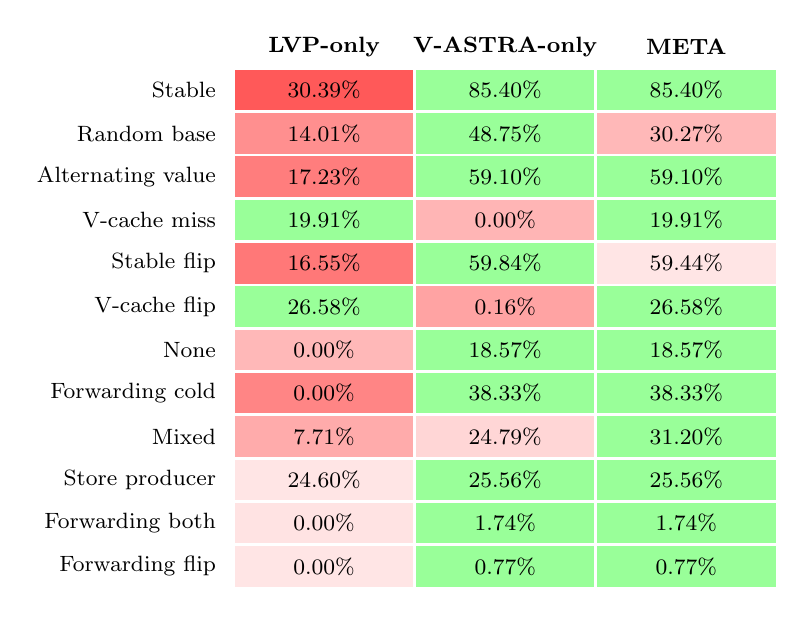
\begin{tikzpicture}[cell/.style={draw=white, line width=1pt,
        minimum width=2.30cm, minimum height=0.55cm, font=\footnotesize}]
    \node[font=\footnotesize\bfseries] at (4.15,0) {LVP-only};
    \node[font=\footnotesize\bfseries] at (6.45,0) {V-ASTRA-only};
    \node[font=\footnotesize\bfseries] at (8.75,0) {META};
    \node[anchor=east, font=\footnotesize] at (2.9,-0.55) {Stable};
    \node[cell, fill=red!65] at (4.15,-0.55) {30.39\%};
    \node[cell, fill=green!40] at (6.45,-0.55) {85.40\%};
    \node[cell, fill=green!40] at (8.75,-0.55) {85.40\%};
    \node[anchor=east, font=\footnotesize] at (2.9,-1.10) {Random base};
    \node[cell, fill=red!44] at (4.15,-1.10) {14.01\%};
    \node[cell, fill=green!40] at (6.45,-1.10) {48.75\%};
    \node[cell, fill=red!28] at (8.75,-1.10) {30.27\%};
    \node[anchor=east, font=\footnotesize] at (2.9,-1.65) {Alternating value};
    \node[cell, fill=red!51] at (4.15,-1.65) {17.23\%};
    \node[cell, fill=green!40] at (6.45,-1.65) {59.10\%};
    \node[cell, fill=green!40] at (8.75,-1.65) {59.10\%};
    \node[anchor=east, font=\footnotesize] at (2.9,-2.20) {V-cache miss};
    \node[cell, fill=green!40] at (4.15,-2.20) {19.91\%};
    \node[cell, fill=red!29] at (6.45,-2.20) {0.00\%};
    \node[cell, fill=green!40] at (8.75,-2.20) {19.91\%};
    \node[anchor=east, font=\footnotesize] at (2.9,-2.75) {Stable flip};
    \node[cell, fill=red!53] at (4.15,-2.75) {16.55\%};
    \node[cell, fill=green!40] at (6.45,-2.75) {59.84\%};
    \node[cell, fill=red!10] at (8.75,-2.75) {59.44\%};
    \node[anchor=east, font=\footnotesize] at (2.9,-3.30) {V-cache flip};
    \node[cell, fill=green!40] at (4.15,-3.30) {26.58\%};
    \node[cell, fill=red!36] at (6.45,-3.30) {0.16\%};
    \node[cell, fill=green!40] at (8.75,-3.30) {26.58\%};
    \node[anchor=east, font=\footnotesize] at (2.9,-3.85) {None};
    \node[cell, fill=red!28] at (4.15,-3.85) {0.00\%};
    \node[cell, fill=green!40] at (6.45,-3.85) {18.57\%};
    \node[cell, fill=green!40] at (8.75,-3.85) {18.57\%};
    \node[anchor=east, font=\footnotesize] at (2.9,-4.40) {Forwarding cold};
    \node[cell, fill=red!48] at (4.15,-4.40) {0.00\%};
    \node[cell, fill=green!40] at (6.45,-4.40) {38.33\%};
    \node[cell, fill=green!40] at (8.75,-4.40) {38.33\%};
    \node[anchor=east, font=\footnotesize] at (2.9,-4.95) {Mixed};
    \node[cell, fill=red!33] at (4.15,-4.95) {7.71\%};
    \node[cell, fill=red!16] at (6.45,-4.95) {24.79\%};
    \node[cell, fill=green!40] at (8.75,-4.95) {31.20\%};
    \node[anchor=east, font=\footnotesize] at (2.9,-5.50) {Store producer};
    \node[cell, fill=red!10] at (4.15,-5.50) {24.60\%};
    \node[cell, fill=green!40] at (6.45,-5.50) {25.56\%};
    \node[cell, fill=green!40] at (8.75,-5.50) {25.56\%};
    \node[anchor=east, font=\footnotesize] at (2.9,-6.05) {Forwarding both};
    \node[cell, fill=red!11] at (4.15,-6.05) {0.00\%};
    \node[cell, fill=green!40] at (6.45,-6.05) {1.74\%};
    \node[cell, fill=green!40] at (8.75,-6.05) {1.74\%};
    \node[anchor=east, font=\footnotesize] at (2.9,-6.60) {Forwarding flip};
    \node[cell, fill=red!10] at (4.15,-6.60) {0.00\%};
    \node[cell, fill=green!40] at (6.45,-6.60) {0.77\%};
    \node[cell, fill=green!40] at (8.75,-6.60) {0.77\%};
    \end{tikzpicture}
    \caption{Cycle reduction relative to NP for LVP-only, V-ASTRA-only,
    and META (\texttt{metaAstraLvpLoads=off}). Green marks the largest
    reduction for each workload. Red shading grows with the gap, in
    percentage points, to that largest reduction.}
    \label{tab:meta-cycle-comparison}
\end{figure}

META matches the better of the two predictors on nine of the twelve
workloads, and on mixed it beats both, with a 31.20\% reduction. Mixed
is where combining helps most, because LVP serves one part of the lap
and V-ASTRA the other. On random base and stable flip, however, META
is slower than V-ASTRA alone: 24,828 versus 18,249 cycles on random
base, and 13,039 versus 12,912 on stable flip. So combining the
predictors does not always give the best result. These measurements
alone do not explain every difference, but the random-base case is
examined in the next subsection.

\subsection{Provisional-Base Modes on the Random-Base Workload}
\label{subsec:provisional-base-performance}

To find out why META loses on random base, I ran it in all three
modes of Section~\ref{sec:impl-provisional}.
Figure~\ref{tab:randbase-mode-cycles} shows the cycle reductions and
L1D read misses.

\begin{figure}[H]
    \centering
    \pgfplotsset{rbmode/.style={perfbar, width=0.52\linewidth, height=5.4cm,
        bar width=13pt, enlarge x limits=0.13,
        symbolic x coords={NP,V-ASTRA,off,train,candidate},
        xticklabels={No pred.,V-ASTRA,META off,META train,META cand.},
        xticklabel style={rotate=35, anchor=north east, font=\footnotesize}}}
    \begin{tikzpicture}
    \begin{axis}[rbmode, ymax=60, ylabel={Cycle reduction vs NP (\%)},
        nodes near coords={\pgfmathprintnumber[fixed,precision=2]{\pgfplotspointmeta}}]
        \addplot[fill=metac, draw=metac!70!black] coordinates
            {(NP,0) (V-ASTRA,48.75) (off,30.27) (train,30.57) (candidate,50.80)};
    \end{axis}
    \end{tikzpicture}\hfill
    \begin{tikzpicture}
    \begin{axis}[rbmode, ymax=950, ylabel={L1D read misses}]
        \addplot[fill=candc, draw=candc!70!black] coordinates
            {(NP,800) (V-ASTRA,205) (off,591) (train,587) (candidate,182)};
    \end{axis}
    \end{tikzpicture}
    \caption{Random-base cycle reduction relative to NP (left) and L1D
    read misses (right) across provisional-base modes.}
    \label{tab:randbase-mode-cycles}
\end{figure}

Figure~\ref{tab:randbase-mode-events} shows the matching event
counts. In this workload, every V-ASTRA candidate also bypassed, so
the candidate count equals the number of bypasses.

\begin{figure}[H]
    \centering
    \begin{tikzpicture}
    \begin{axis}[perfbar, width=0.95\linewidth, height=5.4cm,
        bar width=9pt, ymax=760, enlarge x limits=0.15,
        every node near coord/.append style={font=\tiny, rotate=90, anchor=west},
        ylabel={Count},
        symbolic x coords={V-ASTRA-only,META off,META train,META candidate}]
        \addplot[fill=vac, draw=vac!70!black] coordinates
            {(V-ASTRA-only,595) (META off,209) (META train,213) (META candidate,618)};
        \addplot[fill=lvpc, draw=lvpc!70!black] coordinates
            {(V-ASTRA-only,0) (META off,386) (META train,386) (META candidate,182)};
        \addplot[fill=candc, draw=candc!70!black] coordinates
            {(V-ASTRA-only,0) (META off,0) (META train,386) (META candidate,182)};
        \addplot[fill=npc, draw=npc!70!black] coordinates
            {(V-ASTRA-only,0) (META off,386) (META train,0) (META candidate,0)};
        \legend{V-ASTRA candidates, LVP committed loads,
                Provisional bases, Base unavailable}
    \end{axis}
    \end{tikzpicture}
    \caption{Random-base event counts. Every provisional base was
    validated and none was dropped. V-ASTRA-only has no LVP.}
    \label{tab:randbase-mode-events}
\end{figure}

In \texttt{off} mode, LVP serves 386 loads, and none of them can
become V-ASTRA candidates. This leaves only 209 candidates, compared
with 595 for V-ASTRA alone. The \texttt{train} mode changes little,
with only 106 fewer cycles than \texttt{off}. The \texttt{candidate}
mode is much faster. It needs 7,310 fewer cycles than \texttt{off}
(29.4\%) and 731 fewer than V-ASTRA alone. It raises the number of
bypasses from 209 to 618, cuts L1D read misses from 591 to 182, and
reduces the loads served by LVP from 386 to 182.

\subsection{Performance of Dependency-Handling Designs}
\label{subsec:dependency-performance}

These experiments use the default timing (\texttt{extraAssumedLat =
2}), so Design~A has no effect here and is not measured. Design~B is
turned on together with V-ASTRA, and there was no V-ASTRA run without
forwarding to compare against. Figure~\ref{tab:forwarding-performance} shows V-ASTRA with
forwarding against NP on the four forwarding workloads. The number
under each workload counts loads admitted to forwarding, not
committed instructions.

\begin{figure}[H]
    \centering
    \begin{tikzpicture}
    \begin{axis}[perfbar, width=0.85\linewidth, height=5.2cm,
        bar width=22pt, ymax=45, enlarge x limits=0.18,
        ylabel={Cycle reduction vs NP (\%)},
        symbolic x coords={fc,mx,fb,ff},
        xticklabels={{Forwarding cold\\(188 fwd.)},{Mixed\\(188 fwd.)},
                     {Forwarding both\\(400 fwd.)},{Forwarding flip\\(394 fwd.)}},
        xticklabel style={align=center},
        nodes near coords={\pgfmathprintnumber[fixed,precision=2]{\pgfplotspointmeta}\%}]
        \addplot[fill=vac, draw=vac!70!black] coordinates
            {(fc,38.33) (mx,24.79) (fb,1.74) (ff,0.77)};
    \end{axis}
    \end{tikzpicture}
    \caption{Cycle reduction of V-ASTRA with forwarding relative to NP on
    the forwarding workloads. The number under each workload is the
    number of loads admitted to forwarding.}
    \label{tab:forwarding-performance}
\end{figure}

On forwarding cold, cycles drop by 38.33\%, yet L1D read misses stay
at 400, even with 191 bypasses. The gain seems to come from
overlapping the cold misses rather than from avoiding them, although
the measurements cannot isolate this. On forwarding both and
forwarding flip, the gains are small (1.74\% and 0.77\%), with a
run-to-run variation of about 0.06\% and 0.15\% on those workloads.

\subsection{Threats to Validity and Interpretation}
\label{subsec:performance-limitations}

These results come from small deterministic microbenchmarks on one
MinorCPU, cache, and memory configuration, so they are not
application-level speedups. The repeated runs only test sensitivity to
memory layout, and are not independent statistical samples. Design~A
was not measured under the default timing, and Design~B's share of
the gain cannot be separated from V-ASTRA.

Overall, the cycle reductions are large but depend strongly on the
workload. META beats both predictors on mixed, but is slower than
V-ASTRA alone on random base and stable flip. Candidate mode gives a
large improvement on random base.

\newpage
\section{Limitations and Differences from the Original Paper}

This work adapts the paper's prediction mechanisms to gem5 MinorCPU.
It does not reproduce the paper's full processor or its evaluation
setup~\cite{ravenel2025architecting}. The two differ in the
processor model, in when predictions are checked, and in how
performance is measured.

\subsection{Processor Model and Evaluation Scope}

The paper evaluates a modified CVA6-based processor on SPEC CPU2017
using SimPoints. This work uses gem5 MinorCPU and small targeted
RISC-V microbenchmarks. Both processors are four-wide. The paper's
processor can issue two loads per cycle and has a 32-entry
scoreboard. The MinorCPU setup used here issues at most one memory
instruction per cycle, and its scoreboard tracks every architectural
register~\cite{ravenel2025architecting}. The caches and workloads
also differ. So the cycle reductions reported here describe this
simulator setup and these microbenchmarks only. They are not
application-level speedups and should not be compared directly with
the paper's results.

\subsection{Differences from the Original Design}
\label{subsec:original-design-differences}

\paragraph{LVP and recovery:} The LVP table and its confidence policy
follow the paper~\cite{ravenel2025architecting}. The difference is in
how predictions are used. Here, an LVP prediction can only serve as
the base address of a dependent integer load, and only while its
producer is the oldest instruction and still waiting for its data
(Section~\ref{sec:lvp-integration}). Both the paper and this work
recover only when a wrong prediction was actually used, but the
recovery method differs. The paper replays younger instructions
through its scoreboard, while the implementation squashes them and fetches
them again.

\paragraph{Address and tag compression:} The paper's Last Address
Compressed Table (LACT) is a 32-entry LRU structure that replaces the
upper 44 bits of an address with a 5-bit identifier and keeps only the
lower 20 bits in the predictor. This cuts predictor storage by 85\%.
The value-cache tags reuse the same identifier, which cuts tag
storage by 75\%~\cite{ravenel2025architecting}. This work keeps full
64-bit bases and full page-number tags instead. The value cache has
the same 4\,KiB capacity and 16-byte entries as the paper's, but it
tracks validity per byte, does not fill whole 16-byte lines.

\paragraph{When V-ASTRA is checked:} The paper validates the predicted
base at issue, so dependents can issue in the same cycle as the load.
Here, the base is checked in Execute when the load forms its address,
and the bypass is accepted later in the LSQ, after address translation
and some of the safety checks (Section~\ref{sec:impl-vcache}).

\paragraph{Store safety:} The paper tracks possible conflicts with
older stores using a counting Bloom filter and an invalidation
FIFO~\cite{ravenel2025architecting}. This work scans the older
in-flight stores exactly, both when forming a candidate and again
before the bypass. An exact scan avoids the Bloom filter's false
positives, but its cost grows with the number of in-flight stores.
The FIFO is not needed here. Memory operations enter the LSQ in
order, so older store addresses are already known at the decision
point.

\paragraph{L0 minicache:} The paper's L0 minicache is a 32-entry
direct-mapped structure with speculative and committed data. It lets
loads blocked by in-flight stores still be served
quickly~\cite{ravenel2025architecting}. It is not implemented here.
Such loads fall back to the normal memory path, where MinorCPU's
store buffer forwards fully covered loads and makes partly covered
ones wait.

\paragraph{Dependency handling:} In the paper, dependents of a
validated load can issue and execute in the same cycle. In MinorCPU,
non-memory instructions still execute at commit. Design~A only lets
dependents issue earlier under stall-on-use timing, and it has no
effect under the default timing. Design~B forwards a validated value,
but only to the base address of a dependent integer load, not to ALU,
branch, store, or floating-point instructions.

\subsection{Future Work}

\paragraph{Extending this work:} The random-base result suggests a
smarter rule for when an LVP-supplied base may be used for V-ASTRA,
for example based on LVP confidence, recent validation results, or
agreement with ASTRA. Such a rule should be tested on random base,
stable flip, V-cache flip, mixed, and the forced-misprediction
workload, to check both gains and regressions. Design~B should be
measured on its own, by comparing V-ASTRA with and without
forwarding, and Design~A should be measured under stall-on-use
timing. Design~B could also forward to other load operands and to
store addresses. Forwarding to ALU and branch instructions would need
larger changes to MinorCPU.

\paragraph{Closer to the paper:} The biggest missing piece is the
L0 minicache, which would give a fast path to loads that V-ASTRA
currently rejects because of in-flight stores. It would need LSQ
integration, speculative store handling, line locking, and recovery,
and it should be evaluated on store-heavy workloads together with
META. Adding LACT-style compression
(Section~\ref{subsec:original-design-differences}) would mainly reduce
storage. It would need identifier allocation and recycling,
compressed tables and tags, cache invalidation when identifiers are
reused, and a check for displacements that cross the compressed
region. Replacing the exact store scan with a Bloom filter, or
squash-and-refetch with scoreboard replay, would bring the design
closer to the paper but is lower priority. The paper also discusses
VTAGE, process-ID-tagged value-cache entries, multiprocessor support,
and security~\cite{ravenel2025architecting}.

\paragraph{Broader evaluation:} The current results use deterministic
microbenchmarks and one processor and memory configuration. Future
evaluations should use application-level and embedded benchmarks,
other cache and memory-latency settings, and other processor widths
where possible. Supporting compressed RISC-V loads would allow
binaries built for \texttt{rv64gc}.

\newpage
\section{Conclusion}

In this project, I added value prediction to gem5's MinorCPU. The
implementation includes Last Value Prediction (LVP), the ASTRA base
predictor, a separate value cache, and a guarded V-ASTRA bypass that
lets a load skip memory when its safety checks pass. I also tried two
ways of letting dependents start earlier. Design~A only releases the
scoreboard dependency, and Design~B also forwards the validated value
to a dependent load. On top of these, I adapted the paper's META to
choose, for each dependent load, at most one of the V-ASTRA value and
the LVP prediction. A load waits while the V-ASTRA outcome is still
pending. An experimental option lets loads served by LVP pass their
bases to ASTRA for training and for V-ASTRA candidacy.

The results depend strongly on the workload. META gives a 31.20\%
cycle reduction on the mixed workload, more than either predictor
alone. On random base, however, default META reaches only 30.27\%,
compared with 48.75\% for V-ASTRA alone. This is most likely because
the loads served by LVP can no longer become V-ASTRA candidates. META
is also slightly slower than V-ASTRA on stable flip. The experimental
candidate mode gives these loads back to V-ASTRA and raises the
random-base reduction to 50.80\%, but it did not change the cycle
count on mixed or V-cache miss. These numbers describe small
microbenchmarks on one simulated configuration, not application
speedups. Design~A was validated but not performance-tested under
stall-on-use, and Design~B's share of the gain could not be separated
from V-ASTRA.

Directed tests covered the predictors, the value cache, memory
ordering, dependency handling, and recovery. They showed that a wrong
LVP prediction needs recovery only if it was used, and that loads
served by V-ASTRA never trigger LVP recovery. They also exposed a
cleanup bug after early alignment faults, which I then fixed. A
complete regression of all suites on the final source passed with no
failures.

Overall, the project shows how many parts of an in-order pipeline
value prediction touches. Speculative operands, address prediction,
the value-cache bypass, memory ordering, dependency tracking, and
recovery all have to work together. It gives a working base for
further study in MinorCPU. The most useful next steps are the L0
minicache and LACT compression from the paper, a smarter rule for
when LVP-served bases may become candidates, and evaluation on more
realistic workloads.


\section*{Acknowledgements}

\begin{enumerate}
    \item I thank my project guide, \textbf{Prof.\ Gopalakrishnan Srinivasan},
    and my mentor, \textbf{Girinath}, for their guidance and feedback
    throughout this project.

    \item I used AI assistant (Claude, by Anthropic) during the
    project. It helped with parts of the implementation and test
    scripts, and with setting up and running the regression suite. I have crosschecked the code produced and ensured that the implementation matches with project's design. I have checked the workloads and the results myself. It
    was also used to format the report in \LaTeX{}, improving the readability at some places and was used to make
    diagrams and figures.
\end{enumerate}

\bibliographystyle{plain}
\bibliography{references}

\end{document}
